\chapter{ワークB 脈拍測定プログラム開発}

\section{はじめに}
% 本ワークの目的
マイクロコントローラ（マイコン）を用いた生体計測システムでは，センサ回路から出力されるアナログ電気信号をA/Dコンバータ（ADC）によりデジタル値へ変換し，プログラムによる信号処理を通じて所望の特徴量を抽出・出力する一連のデータ処理系を構築することが求められる．
本実習（ワークB）の目的は，脈拍測定プログラムの開発を通して，マイコン（Arduino Uno R4 WiFi）へのアナログ入力，入力データの信号処理，および処理結果のシリアル出力といったマイコンを用いた一連のデータ処理方法について理解を深めるとともに，開発したシステムが目的の機能・性能を果たしているかを実験データに基づき客観的に検証・報告することである\cite{elgendi2019use, 安藤譲二1990光電式脈波計測の応用}．
本実習は以下の3つの段階で構成される：
\begin{enumerate}
  \item \textbf{ワークB-1（信号波形の入力と確認）}：波形出力デバイス（M5Stack ATOM Lite）に記録された4種類の信号波形をArduinoのADCを用いて読み込み，図示しやすいCSV形式でシリアル出力するプログラムを開発し，描画したグラフの波形特徴からどの信号波形が脈波を表すかを特定する．
  \item \textbf{ワークB-2（ピーク検出プログラムの作成）}：脈波信号のAD変換値から拍動の頂点（ピーク）を検出して一括出力するプログラムを作成し，山領域を判定する閾値（\texttt{TOP\_THRESHOLD}）と下降傾向を判定する閾値（\texttt{DOWN\_THRESHOLD}）の組み合わせを系統的に変化させて最適な閾値を決定する．
  \item \textbf{ワークB-3（脈拍測定プログラムの作成）}：決定した最適閾値によるピーク検出を基に，連続する2点のピーク間隔（拍動周期）から1分間あたりの脈拍数（bpm）を算出する関数（\texttt{rate}関数）を実装し，測定結果の基本統計値および生理的意味について考察する．
\end{enumerate}


\section{ワークB-1}
% ワークB-1の目的と実施内容を記載せよ
ワークB-1の目的は，ATOM Liteに保存された4種類の信号波形をArduinoのADCを利用して読み込み，CSV形式でシリアル出力するプログラムを開発し，可視化した波形の特徴から脈波を表す信号波形を特定することである．
ATOM Liteの5Vピン，Gピン，およびDAC対応ピン（G25）をそれぞれArduino Uno R4 WiFiの5V，GND，およびアナログ入力ピン（A0）へジャンパーワイヤで接続した．
起動時にヘッダー行（\texttt{time,value}）を1度だけ出力し，その後は起動後5秒が経過するまで20\,ms周期で経過時間（秒単位，小数点以下2桁）とAD変換値の組を1行ずつシリアル出力するスケッチ（\texttt{b1\_signal\_check.ino}）を作成した．
ATOM Liteのボタンを押して信号波形とLEDの色（緑，赤，青，紫）を順次切り替えながら，Pythonスクリプト（\texttt{b1\_plot\_graph.py}）を用いてシリアル信号を受信し，各色のCSVファイルおよび波形グラフ（PNGファイル）を作成した．

\subsection{脈波信号の検討}
% 出力した各信号波形の図を参照し，特徴を説明した上で，どの信号波形が脈波なのか結論を述べること
% 根拠について参考にした文献がある場合は，参考文献に追加した上で，説明を記述する際に引用せよ

\begin{figure}[htbp]
  \centering
  \begin{minipage}[b]{0.48\textwidth}
    \centering
    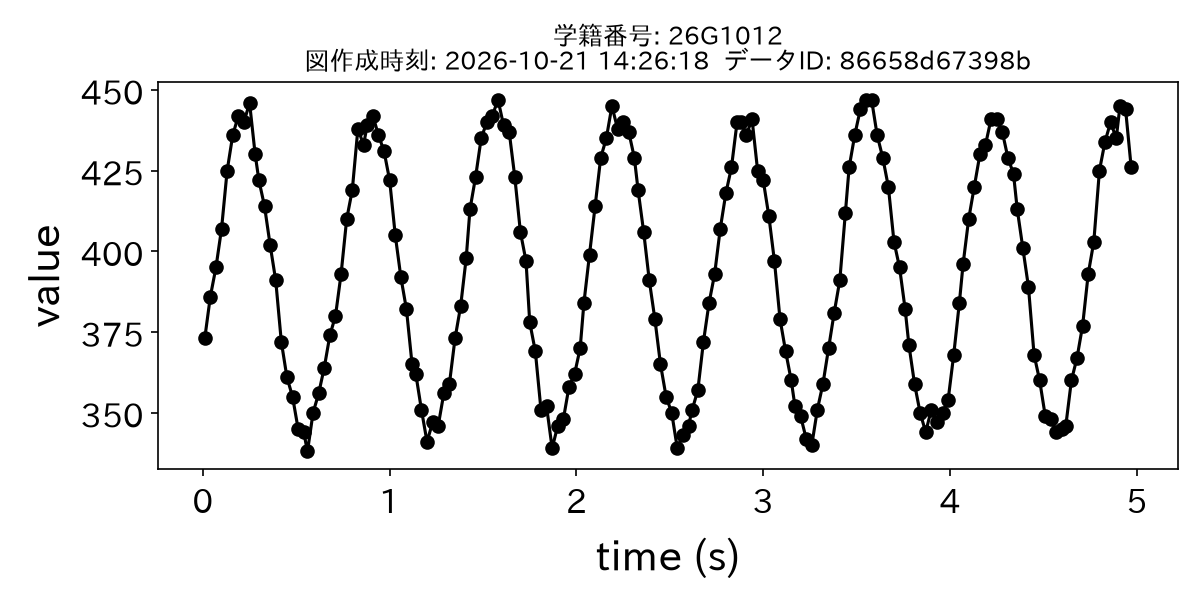
\includegraphics[width=\textwidth]{fig_work_B/b1_26G1012_green_20261021_142618_86658d67398b.png}
    \caption{緑色LED時の出力波形}
    \label{fig:b1_green}
  \end{minipage}
  \hfill
  \begin{minipage}[b]{0.48\textwidth}
    \centering
    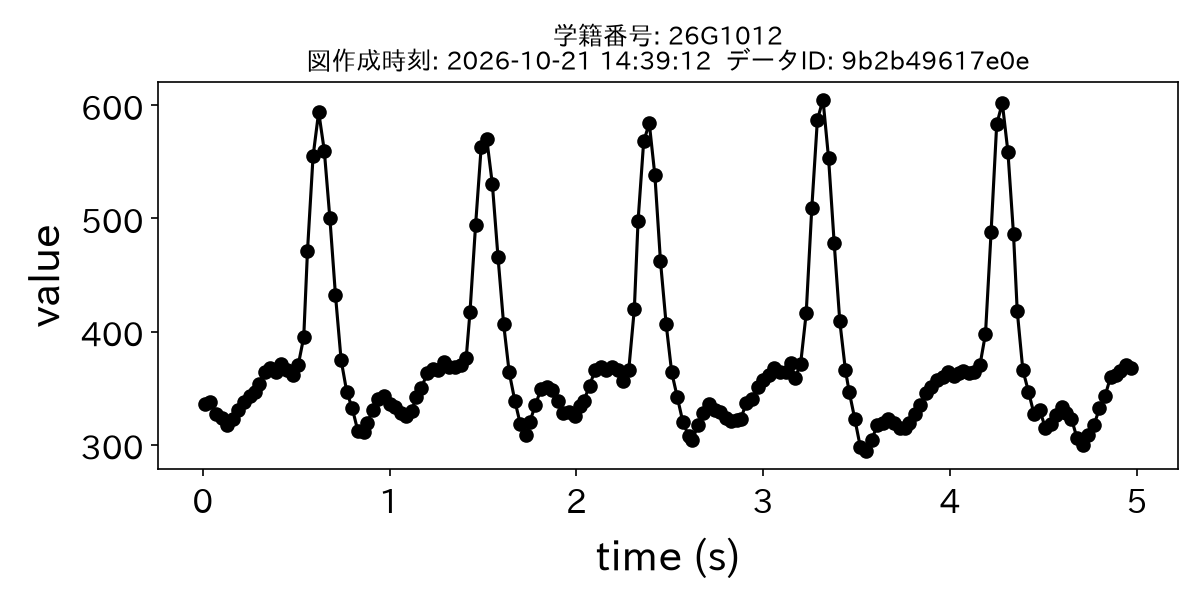
\includegraphics[width=\textwidth]{fig_work_B/b1_26G1012_red_20261021_143912_9b2b49617e0e.png}
    \caption{赤色LED時の出力波形}
    \label{fig:b1_red}
  \end{minipage}
  \vspace{0.8em}
  \begin{minipage}[b]{0.48\textwidth}
    \centering
    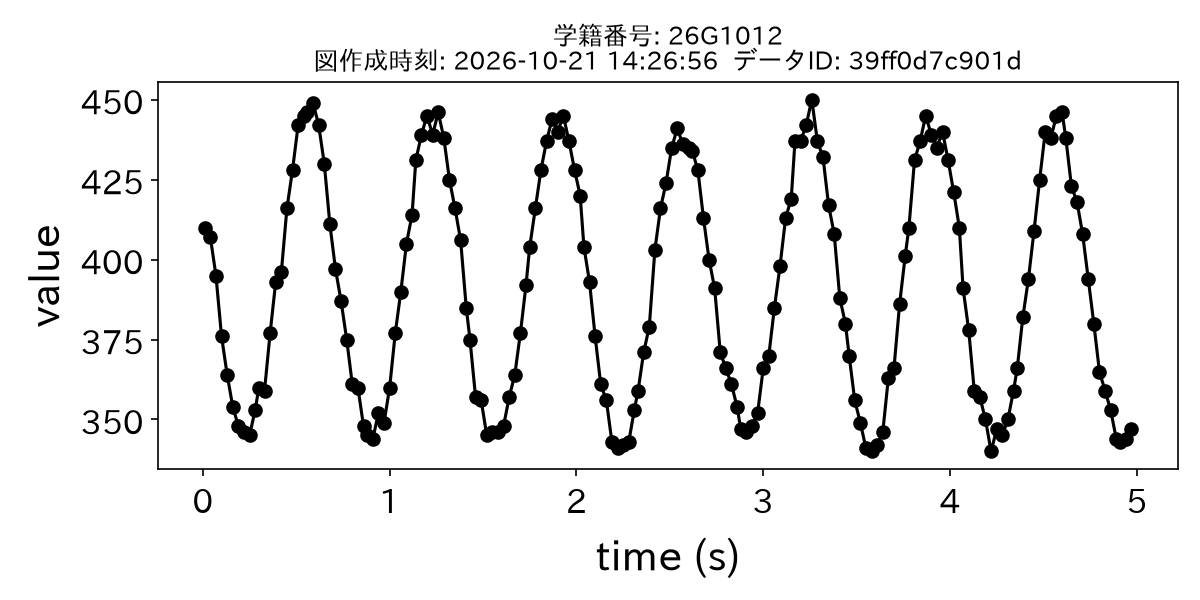
\includegraphics[width=\textwidth]{fig_work_B/b1_26G1012_blue_20261021_142656_39ff0d7c901d.png}
    \caption{青色LED時の出力波形}
    \label{fig:b1_blue}
  \end{minipage}
  \hfill
  \begin{minipage}[b]{0.48\textwidth}
    \centering
    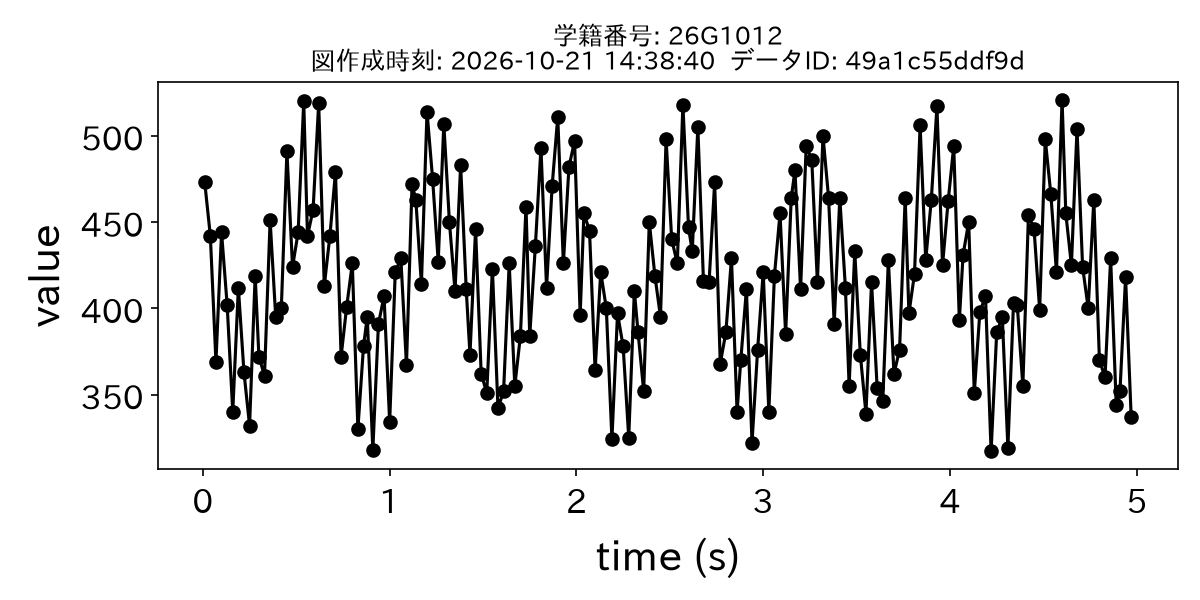
\includegraphics[width=\textwidth]{fig_work_B/b1_26G1012_purple_20261021_143840_49a1c55ddf9d.png}
    \caption{紫色LED時の出力波形}
    \label{fig:b1_purple}
  \end{minipage}
  \caption{ATOM Liteより入力された4種類の信号波形}
  \label{fig:b1_all_waveforms}
\end{figure}

ATOM Liteから出力された4種類の信号波形（緑色，赤色，青色，紫色）を計測・グラフ化した結果を図\ref{fig:b1_all_waveforms}（図\ref{fig:b1_green}〜図\ref{fig:b1_purple}）に示す．
各信号波形の特徴は以下の通りである：
\begin{itemize}
  \item \textbf{緑色LED（図\ref{fig:b1_green}）}：AD変換値が338から447の範囲で周期約0.95\,s（約1\,Hz）にて滑らかに上下する単一周波数の正弦波であり，上限と下限が対称で高調波成分や変曲点を含まない．
  \item \textbf{赤色LED（図\ref{fig:b1_red}）}：基底値（294〜330付近）から急峻に立ち上がって高い主峰ピーク（570〜605）に達した後，緩やかに下降する途中で小さな谷と山（値364〜373付近の変曲点）を経て基底へ戻る，周期約0.9\,sの左右非対称な波形である．
  \item \textbf{青色LED（図\ref{fig:b1_blue}）}：AD変換値が340から450の範囲で周期約0.95\,sにて推移する正弦波状の波形（1\,Hzの基本波に高周波ノイズ成分が重畳し，約20\,ms周期のサンプリングにより折り返されて微細な揺らぎとして現れた波形）であり，鋭い主峰ピークや非対称な減衰特性は認められない．
  \item \textbf{紫色LED（図\ref{fig:b1_purple}）}：約1\,Hzの低周波正弦波に約7\,Hzの中周波正弦波が合成され，AD変換値317から521の範囲で1周期内に多数の小山が等間隔に並んだ合成波であり，生体の拍動波形とは形状が大きく異なる．
\end{itemize}

光電容積脈波に関する文献によれば，末梢動脈における脈波波形は，左心室の収縮期に血液が駆出されることで急峻に立ち上がる主波（収縮期峰：Systolic Peak）と，大動脈弁の閉鎖に伴う一時的な逆流および末梢血管からの反射波によって下降脚の途中に現れる重複切痕（ディクロティック・ノッチ：Dicrotic Notch）および重複波（拡張期峰：Diastolic Peak）から成る非対称な二峰性形状を特徴とすることが知られている\cite{elgendi2019use, 安藤譲二1990光電式脈波計測の応用}．
図\ref{fig:b1_green}〜図\ref{fig:b1_purple}を比較すると，急峻な立ち上がりを示す主波と下降過程における重複切痕・重複波の特徴を明確に有しているのは図\ref{fig:b1_red}のみである．
以上の根拠より，赤色LED（図\ref{fig:b1_red}）の信号波形が脈波を表す信号波形であると結論付けた．

\subsection{実装内容}
% ファイルごとにプログラムを記載し，変更・追加した処理について説明すること（ipynbファイルは必要ない）
% 変更しなかったファイルについては，変更していないことを説明すること

ワークB-1で作成した \texttt{b1\_signal\_check.ino} のプログラムをソースコード\ref{b1_signal_check}に示す．
配布された初期プログラムでは，\texttt{loop}関数内でA0ピンのAD変換値と \texttt{millis()} によるミリ秒単位の経過時間をそれぞれ別々の行に改行付きで無期限に出力する構成であったため，仕様を満たすように以下の変更および追加を行った：
\begin{itemize}
  \item \textbf{CSVヘッダー行の初期出力処理の追加}（3行目）：プログラム実行開始時に \texttt{time,value} というヘッダー文字列を改行付きで1度だけ出力する仕様（仕様2）を満たすため，起動時に1回のみ実行される \texttt{setup}関数内に \texttt{Serial.println("time,value");} を追加した．
  \item \textbf{秒単位への時間換算と5秒間の出力制限処理の実装}（7--8行目，16行目）：経過時間を秒単位の実数として扱うとともに起動後5秒経過以降はシリアル出力を停止する仕様（仕様3，仕様4）を満たすため，\texttt{millis()} で取得したミリ秒値を \texttt{1000.0} で除算して \texttt{float} 型変数 \texttt{t} に保持する処理へ変更した（7行目）．さらに \texttt{if (t < 5.0)} の条件分岐（8行目，16行目）を追加し，経過時間が5秒未満の間のみアナログ値の読み取り・出力および20\,ms待機を実行するように変更した．
  \item \textbf{カンマ区切り（CSV形式）による1行出力への変更}（11--13行目）：経過時間（小数点以下2桁）とアナログ入力値の組をカンマ区切りで1行ずつ出力する仕様（仕様3）を満たすため，\texttt{Serial.print(t, 2);} により経過時間を小数点以下2桁かつ改行なしで出力し（11行目），\texttt{Serial.print(",");} で区切り文字を出力した後に（12行目），\texttt{Serial.println(v);} でアナログ値 \texttt{v} を改行付きで出力する処理へ変更した（13行目）．
\end{itemize}

\begin{figure}[H]
  \begin{lstlisting}[caption=b1\_signal\_check.ino, label=b1_signal_check, escapechar=\@]
void setup() {
  Serial.begin(9600);
  Serial.println("time,value");
}

void loop() {
  float t = millis() / 1000.0;
  if (t < 5.0) {
    uint16_t v = analogRead(A0);

    Serial.print(t, 2);
    Serial.print(",");
    Serial.println(v);

    delay(20);
  }
}
    \end{lstlisting}
\end{figure}


\section{ワークB-2}
% ワークB-2の目的と実施内容を記載せよ
ワークB-2の目的は，ワークB-1で脈波と特定した信号波形をArduinoのADCで読み込み，脈波のピーク（山の頂点）を検出してCSV形式でシリアル出力するプログラムを作成するとともに，山と判定する閾値（\texttt{TOP\_THRESHOLD}）および減少に転じたと判定する閾値（\texttt{DOWN\_THRESHOLD}）について最適な値を実験的に検討・決定することである．
ピーク検出関数 \texttt{top()} 内において，1回の探索ループ中に計測した時刻とAD変換値を配列に蓄積し，ピーク確定または探索終了後にピーク位置フラグ（ピーク時は \texttt{1}，それ以外は \texttt{0}）を付与して一括出力するプログラムを実装した．
その上で，\texttt{TOP\_THRESHOLD} と \texttt{DOWN\_THRESHOLD} の組み合わせを変えてCSVファイルとグラフ（PNGファイル）を作成し，検出性能の比較評価を行った．

\subsection{閾値の検討}
% TOP_THRESHOLDとDOWN_THRESHOLDの組み合わせに応じたグラフと表を基に検討を行い，最終的な閾値がなぜ最適であるかを考察すること
% 最初に，DOWN=0と4，TOP=350と500の4条件で計測を行い，その結果を基に各閾値が検出結果に与える影響を確認
% 次に以下の表に沿って計測と検討を行い，最終的な閾値を決定すること

ピーク検出アルゴリズムでは，入力値 \texttt{value} が \texttt{TOP\_THRESHOLD} 以上の領域において最大値 \texttt{maximum} の更新回数を \texttt{up\_count}，非更新（下降または横ばい）回数を \texttt{down\_count} として計数し，上昇傾向（\texttt{up\_count > UP\_THRESHOLD}）を確認した後に \texttt{down\_count > DOWN\_THRESHOLD}（すなわち頂点通過後に \texttt{TOP\_THRESHOLD} 以上を維持したまま \texttt{DOWN\_THRESHOLD + 1} サンプルの非更新）を満たした時点で保持していた最大値をピークとして確定する．

まず，各閾値が検出結果に与える基本的な影響を確認するため，$\mathrm{DOWN} = 0, 4$，$\mathrm{TOP} = 350, 500$ の4条件で計測を実施した．得られたグラフを図\ref{fig:b2_initial_4cond}（図\ref{fig:b2_350_0}〜図\ref{fig:b2_500_4}）に示す．

\begin{figure}[htbp]
  \centering
  \begin{minipage}[b]{0.48\textwidth}
    \centering
    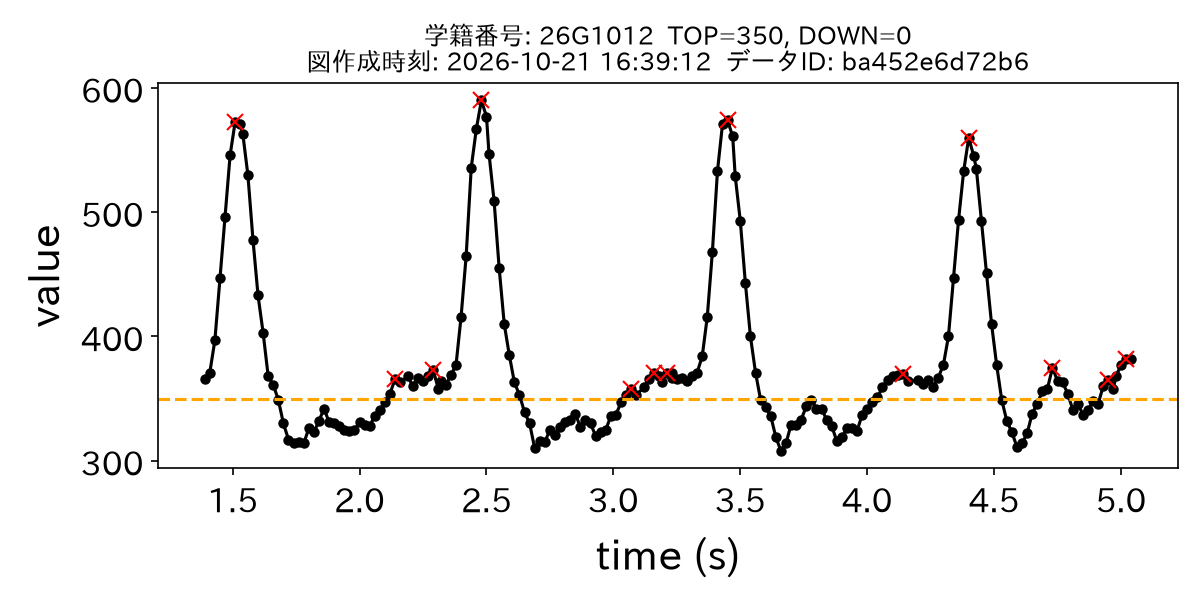
\includegraphics[width=\textwidth]{fig_work_B/b2_26G1012_top350_down0_20261021_163912_ba452e6d72b6.png}
    \caption{$\mathrm{TOP} = 350, \mathrm{DOWN} = 0$（$\times$多）}
    \label{fig:b2_350_0}
  \end{minipage}
  \hfill
  \begin{minipage}[b]{0.48\textwidth}
    \centering
    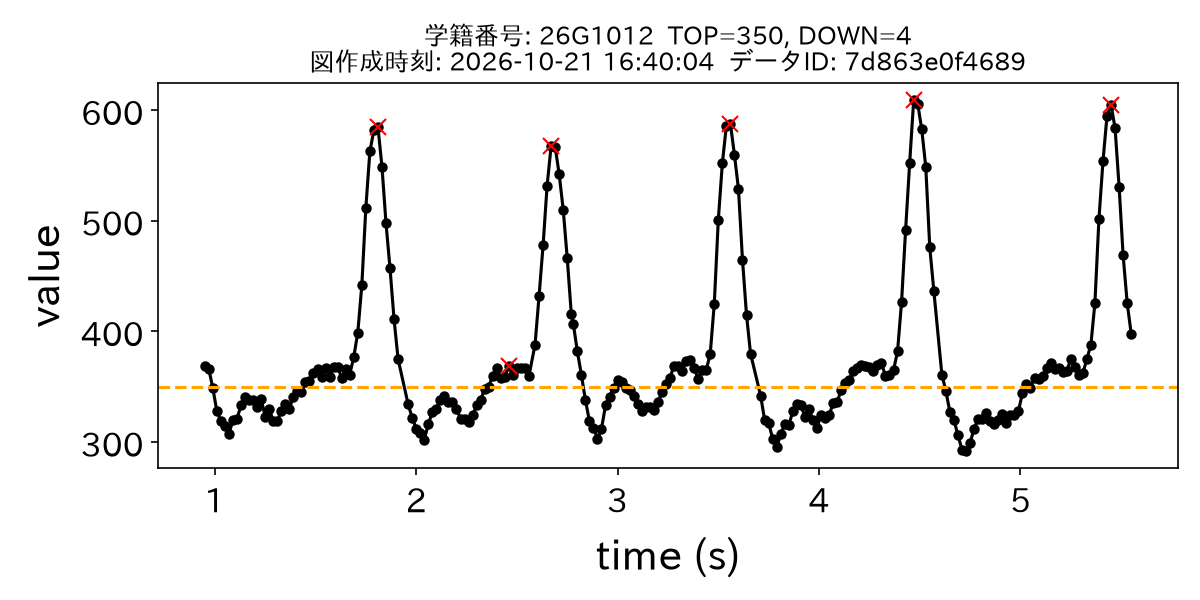
\includegraphics[width=\textwidth]{fig_work_B/b2_26G1012_top350_down4_20261021_164004_7d863e0f4689.png}
    \caption{$\mathrm{TOP} = 350, \mathrm{DOWN} = 4$（$\times$多）}
    \label{fig:b2_350_4}
  \end{minipage}
  \vspace{0.8em}
  \begin{minipage}[b]{0.48\textwidth}
    \centering
    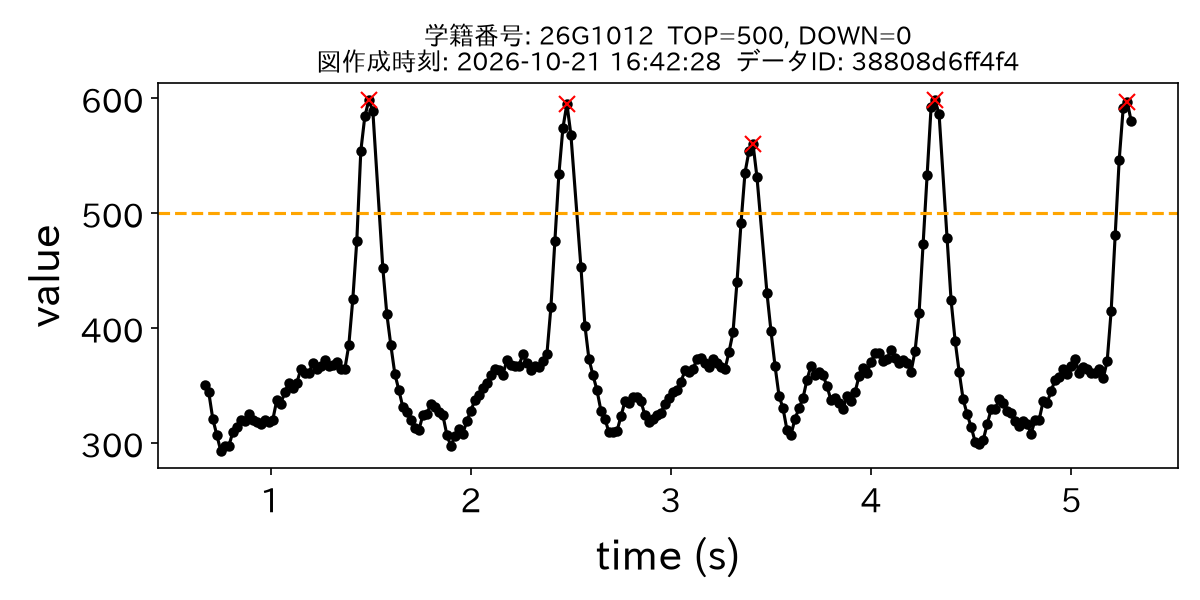
\includegraphics[width=\textwidth]{fig_work_B/b2_26G1012_top500_down0_20261021_164228_38808d6ff4f4.png}
    \caption{$\mathrm{TOP} = 500, \mathrm{DOWN} = 0$（$\bigcirc$）}
    \label{fig:b2_500_0}
  \end{minipage}
  \hfill
  \begin{minipage}[b]{0.48\textwidth}
    \centering
    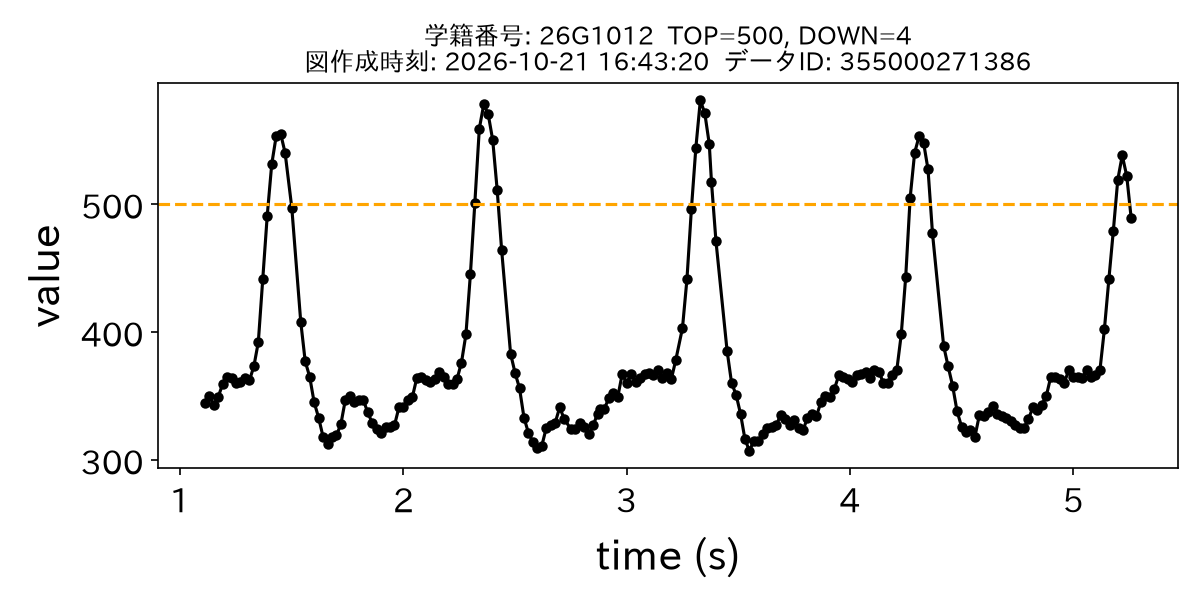
\includegraphics[width=\textwidth]{fig_work_B/b2_26G1012_top500_down4_20261021_164320_355000271386.png}
    \caption{$\mathrm{TOP} = 500, \mathrm{DOWN} = 4$（$\times$漏）}
    \label{fig:b2_500_4}
  \end{minipage}
  \caption{初期4条件（$\mathrm{TOP} \in \{350, 500\}, \mathrm{DOWN} \in \{0, 4\}$）におけるピーク検出結果}
  \label{fig:b2_initial_4cond}
\end{figure}

図\ref{fig:b2_initial_4cond}の4条件の比較から，各閾値が検出結果に与える影響として以下の知見が得られた：
\begin{itemize}
  \item \textbf{$\mathrm{TOP} = 350, \mathrm{DOWN} = 0$（図\ref{fig:b2_350_0}）}：\texttt{TOP\_THRESHOLD} が350と低いため，主波の頂点（560〜590）だけでなく下降脚に現れる重複波（358〜382付近）も山領域として判定された．さらに $\mathrm{DOWN} = 0$ では最大値更新が1サンプル途切れた直後（\texttt{down\_count = 1 > 0}）に即座にピーク確定となるため，重複波の微小な上下動ごとにピークが検出され，1拍動中に最大4回（全体で13回）の複数検出（$\times$多）が発生した．
  \item \textbf{$\mathrm{TOP} = 350, \mathrm{DOWN} = 4$（図\ref{fig:b2_350_4}）}：$\mathrm{DOWN} = 4$ に増やしたことで頂点通過後に350以上の領域で連続5サンプルの非更新が必要となり，図\ref{fig:b2_350_0}で見られた細かな誤検出は大幅に減少した．しかし，重複波の頂点（369〜387）は緩やかに減衰するため，$t = 2.46\,\mathrm{s}$（値369）において5サンプル連続で350以上を維持してしまい，5拍に対して計6個のピークが検出される複数検出（$\times$多）となった．すなわち，重複波を根本的に除外するには \texttt{TOP\_THRESHOLD} を重複波の最大値（約387）より高く設定する必要がある．
  \item \textbf{$\mathrm{TOP} = 500, \mathrm{DOWN} = 0$（図\ref{fig:b2_500_0}）}：\texttt{TOP\_THRESHOLD} を500に設定したことで重複波は探索対象から完全に除外され，かつ $\mathrm{DOWN} = 0$（頂点直後の1サンプル下降で確定）であるため，5拍すべての主峰ピーク（560〜598）が1拍につき1回ずつ検出（$\bigcirc$）された．ただし，$\mathrm{DOWN} = 0$ は上昇途中で1サンプルでもノイズによる停滞・低下が生じるとその時点で誤確定してしまう脆弱性を持つ．
  \item \textbf{$\mathrm{TOP} = 500, \mathrm{DOWN} = 4$（図\ref{fig:b2_500_4}）}：$\mathrm{TOP} = 500$ かつ $\mathrm{DOWN} = 4$ とした場合，頂点通過後に値500以上の領域で5サンプル（約100\,ms）留まり続ける必要がある．しかし，脈波の主峰は急峻であり頂点から2〜3サンプルで500未満へ急落するため，すべての拍動において \texttt{down\_count} が5に達する前に \texttt{value < TOP\_THRESHOLD} の失敗判定に該当し，ピーク検出数は0個（$\times$漏）となった．
\end{itemize}

次に，これらの結果を踏まえ，$\mathrm{TOP} \in \{350, 400, 450, 500\}$，$\mathrm{DOWN} \in \{0, 1, 2, 3, 4\}$ の全20通りの組み合わせについて計測を行った結果を表\ref{tab:threshold_results}に示す．また，閾値の境界挙動を示す代表的な条件（$\mathrm{TOP} = 350, \mathrm{DOWN} = 2$，$\mathrm{TOP} = 400, \mathrm{DOWN} = 4$，$\mathrm{TOP} = 450, \mathrm{DOWN} = 1$，$\mathrm{TOP} = 450, \mathrm{DOWN} = 2$）のグラフを図\ref{fig:b2_comparison}（図\ref{fig:b2_350_2}〜図\ref{fig:b2_450_2}）に，最終的に最適と判断した $\mathrm{TOP} = 400, \mathrm{DOWN} = 2$ のグラフを図\ref{fig:b2_optimal_plot}に示す．

\begin{table}[htbp]
  \centering
  \caption{TOP\_THRESHOLDとDOWN\_THRESHOLDによる検出結果}
  \label{tab:threshold_results}

  \setlength{\tabcolsep}{12pt}
  \renewcommand{\arraystretch}{1.5}

  \begin{tabular}{c|ccccc}
    \hline
    TOP / DOWN & 0          & 1          & 2          & 3          & 4         \\
    \hline
    350        & $\times$多  & $\times$多  & $\times$多  & $\times$多  & $\times$多 \\
    400        & $\bigcirc$ & $\bigcirc$ & $\bigcirc$ & $\bigcirc$ & $\times$漏 \\
    450        & $\bigcirc$ & $\bigcirc$ & $\times$漏  & $\times$漏  & $\times$漏 \\
    500        & $\bigcirc$ & $\bigcirc$ & $\times$漏  & $\times$漏  & $\times$漏 \\
    \hline
  \end{tabular}

  \vspace{1ex}

  \footnotesize
  $\bigcirc$：正常検出，$\times$多：複数検出，$\times$漏：検出漏れ，
  $\times$多・漏：複数検出および検出漏れ，--：未計測
\end{table}

\begin{figure}[htbp]
  \centering
  \begin{minipage}[b]{0.48\textwidth}
    \centering
    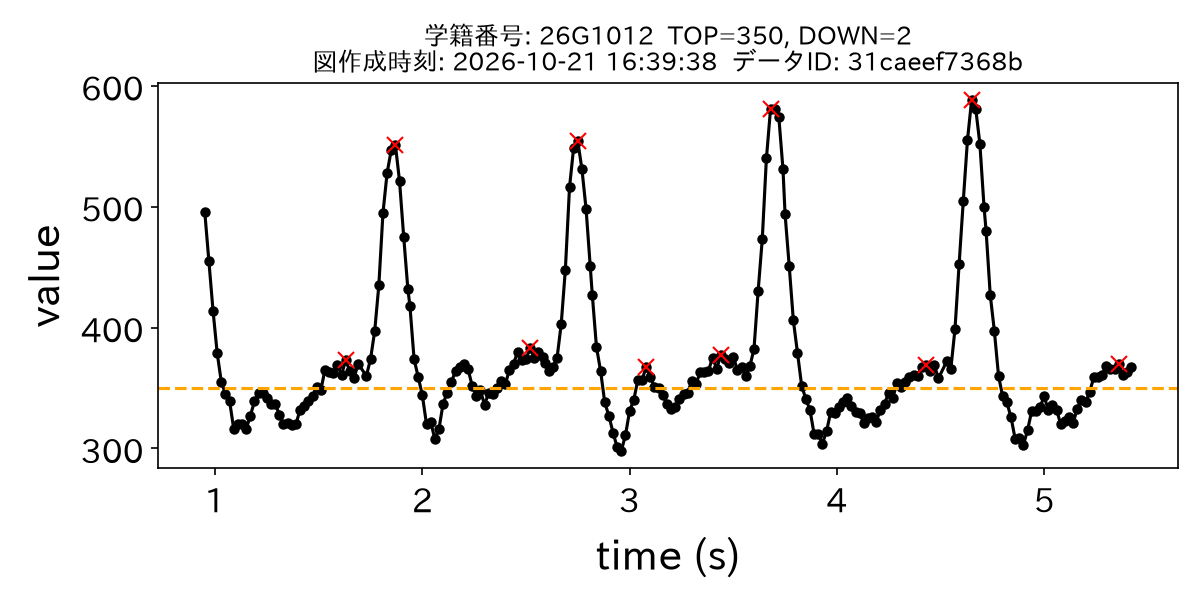
\includegraphics[width=\textwidth]{fig_work_B/b2_26G1012_top350_down2_20261021_163938_31caeef7368b.png}
    \caption{$\mathrm{TOP} = 350, \mathrm{DOWN} = 2$（$\times$多）}
    \label{fig:b2_350_2}
  \end{minipage}
  \hfill
  \begin{minipage}[b]{0.48\textwidth}
    \centering
    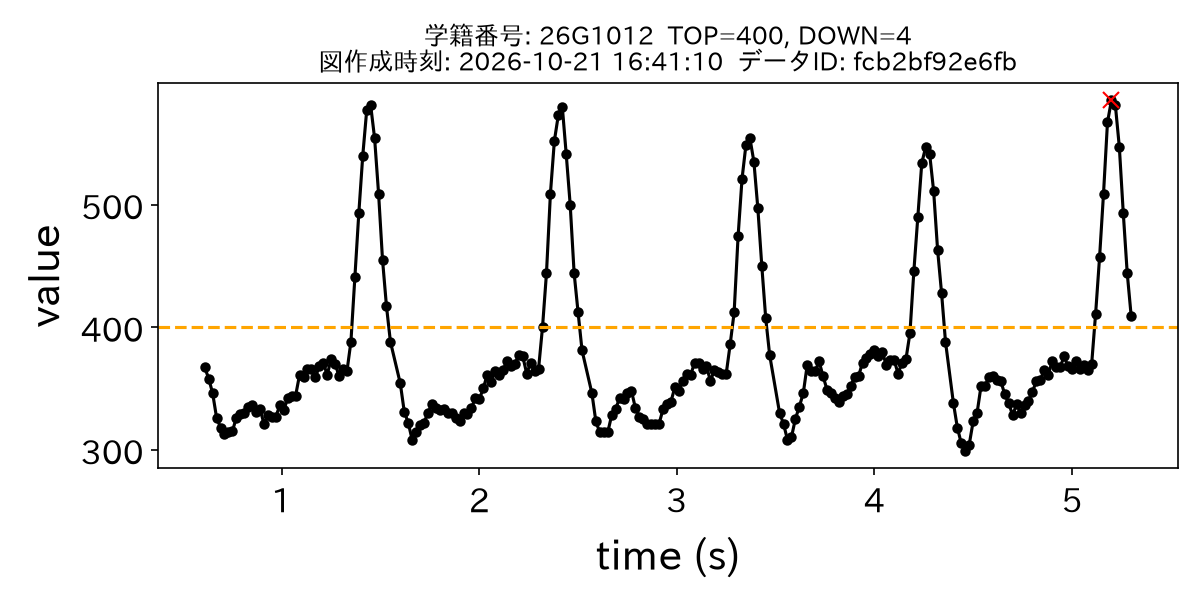
\includegraphics[width=\textwidth]{fig_work_B/b2_26G1012_top400_down4_20261021_164110_fcb2bf92e6fb.png}
    \caption{$\mathrm{TOP} = 400, \mathrm{DOWN} = 4$（$\times$漏）}
    \label{fig:b2_400_4}
  \end{minipage}
  \vspace{0.8em}
  \begin{minipage}[b]{0.48\textwidth}
    \centering
    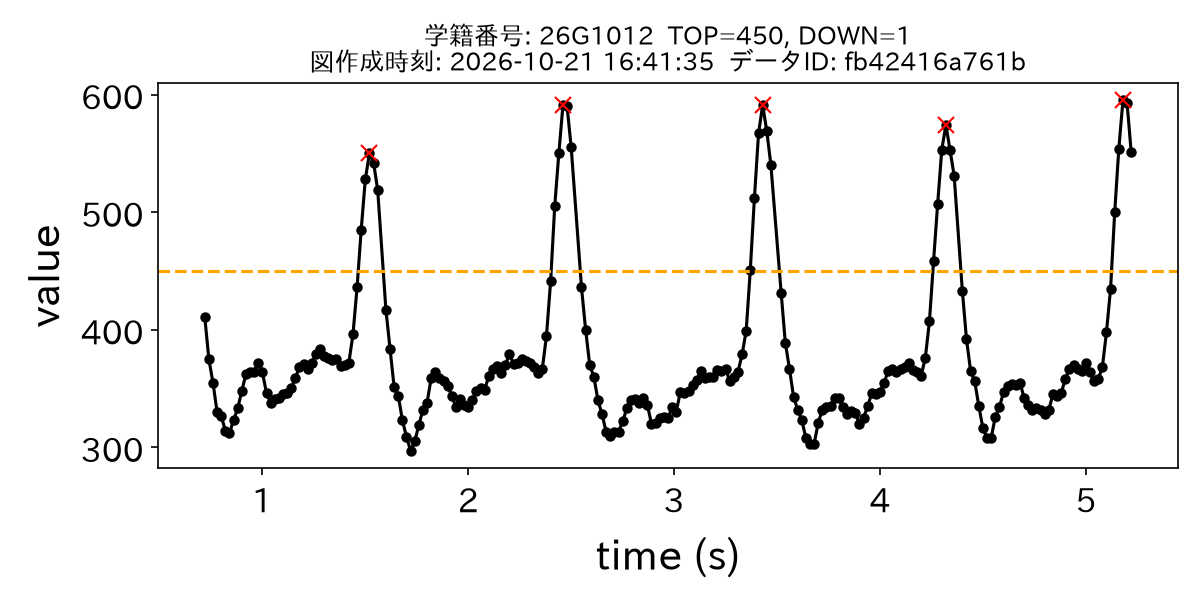
\includegraphics[width=\textwidth]{fig_work_B/b2_26G1012_top450_down1_20261021_164135_fb42416a761b.png}
    \caption{$\mathrm{TOP} = 450, \mathrm{DOWN} = 1$（$\bigcirc$）}
    \label{fig:b2_450_1}
  \end{minipage}
  \hfill
  \begin{minipage}[b]{0.48\textwidth}
    \centering
    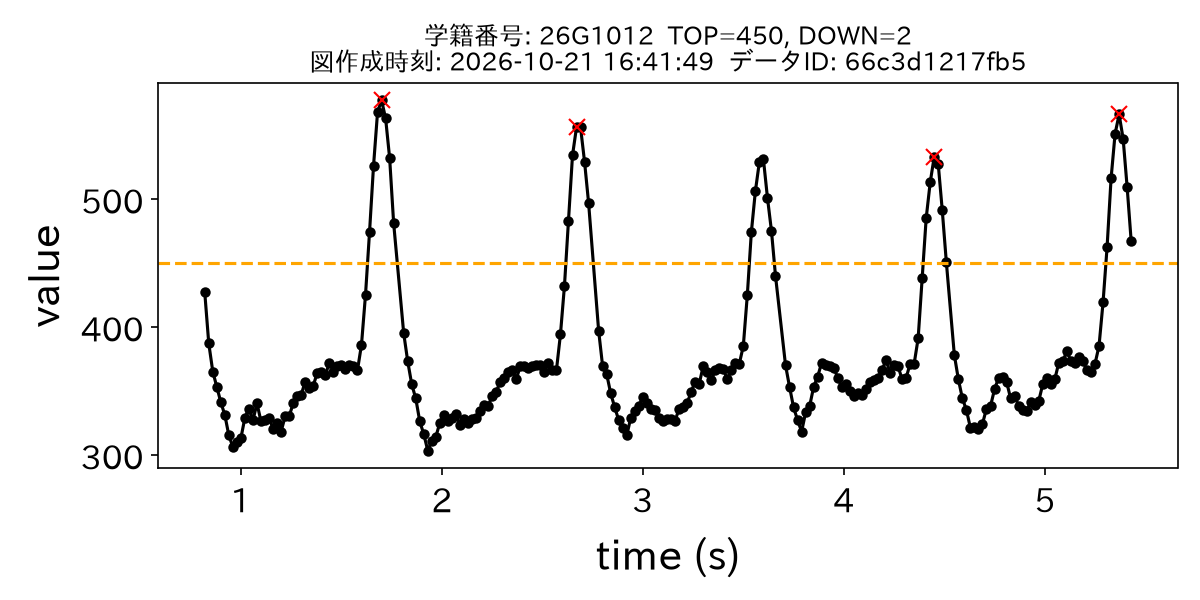
\includegraphics[width=\textwidth]{fig_work_B/b2_26G1012_top450_down2_20261021_164149_66c3d1217fb5.png}
    \caption{$\mathrm{TOP} = 450, \mathrm{DOWN} = 2$（$\times$漏）}
    \label{fig:b2_450_2}
  \end{minipage}
  \caption{各閾値組み合わせにおける境界条件の比較}
  \label{fig:b2_comparison}
\end{figure}

\begin{figure}[htbp]
  \centering
  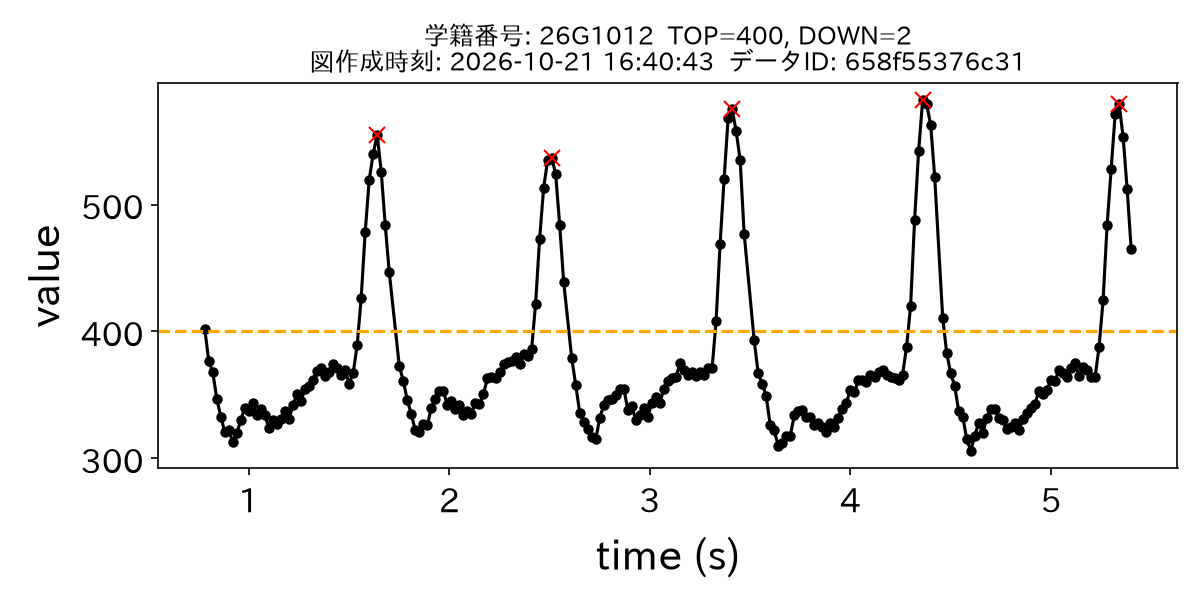
\includegraphics[width=0.75\textwidth]{fig_work_B/b2_26G1012_top400_down2_20261021_164043_658f55376c31.png}
  \caption{最適閾値（$\mathrm{TOP} = 400$, $\mathrm{DOWN} = 2$）におけるピーク検出波形}
  \label{fig:b2_optimal_plot}
\end{figure}

表\ref{tab:threshold_results}および図\ref{fig:b2_comparison}より，以下の検討を行った：
\begin{enumerate}
  \item \textbf{\texttt{TOP\_THRESHOLD} の検討}：
        $\mathrm{TOP} = 350$ では，図\ref{fig:b2_350_2}（$\mathrm{DOWN} = 2$）に見られるように，重複波の極大値（367〜383）が閾値350を上回るため，すべての $\mathrm{DOWN}$ 条件（$0 \sim 4$）において1拍動中に重複波と主波の2箇所が検出される複数検出（$\times$多）となった．
        一方，$\mathrm{TOP} = 450$ および $500$ では，重複波は完全に除外されるものの，閾値が高く主峰の頂点（531〜615）に近いため，頂点通過後に信号値が閾値以上に留まるサンプル数が2サンプル程度と少なくなる．実際に図\ref{fig:b2_450_1}（$\mathrm{TOP} = 450, \mathrm{DOWN} = 1$）では全5拍が正常検出（$\bigcirc$）されたが，図\ref{fig:b2_450_2}（$\mathrm{TOP} = 450, \mathrm{DOWN} = 2$）では $t = 3.60\,\mathrm{s}$ の第3拍（頂点値531）において下降サンプルが $501 \to 475 \to 440$ と推移し，\texttt{down\_count} が3（$> 2$）に達する前に450未満へ脱落して検出漏れ（$\times$漏）が発生した．
        これに対し，$\mathrm{TOP} = 400$ は重複波の最大値（約387）を確実に上回りつつ，主峰頂点との間に130以上の十分な振幅余裕を確保できるため，$\mathrm{DOWN} = 0 \sim 3$ の広い範囲で正常検出（$\bigcirc$）を達成した．

  \item \textbf{\texttt{DOWN\_THRESHOLD} の検討}：
        $\mathrm{TOP} = 400$ において，$\mathrm{DOWN} = 4$（図\ref{fig:b2_400_4}）では頂点通過後に400以上の領域で5サンプル連続の下降が必要となるため，前半4拍（頂点547〜581）で確定前に400を下回り検出漏れ（$\times$漏）となった．
        一方，$\mathrm{DOWN} = 0 \sim 3$ では計測されたすべての拍動ピークが漏れなく1回ずつ検出（$\bigcirc$）された．このうち $\mathrm{DOWN} = 0$ は1サンプルの非更新で確定するため上昇過程での突発的ノイズに弱く，逆に $\mathrm{DOWN} = 3$ は4サンプルの下降確認を要し検出漏れ境界（$\mathrm{DOWN} = 4$）に隣接している．したがって，正常検出領域（$\mathrm{DOWN} = 0 \sim 3$）の中央に位置し，ノイズ耐性と確実なピーク確定の双方に最も高い裕度（マージン）を持つ $\mathrm{DOWN} = 2$（頂点後3サンプル＝約60\,msの連続下降確認）が最適であると判断した．
\end{enumerate}

以上の考察より，最終的な最適閾値を $\mathrm{TOP\_THRESHOLD} = 400$，$\mathrm{DOWN\_THRESHOLD} = 2$ に決定した．図\ref{fig:b2_optimal_plot}に示す通り，この条件では全5拍の主波頂点（値537〜582）のみが赤色の $\times$ 印で過不足なく検出されている．

\subsection{実装内容}
% ファイルごとにプログラムを記載し，変更・追加した処理について説明すること（ipynbファイルは必要ない）
% 変更しなかったファイルについては，変更していないことを説明すること

ワークB-2の実装プログラムをソースコード\ref{b2_peak_detection}，\ref{b2_myPulse.h}，\ref{b2_myPulse.cpp_part1}，および\ref{b2_myPulse.cpp_part2}に示す．

\paragraph{b2\_peak\_detection.ino（ソースコード\ref{b2_peak_detection}）：}
% 変更点の、機能本位での説明を書く。行本位で書かないこと。
配布された初期プログラムでは，\texttt{setup}関数でシリアル通信速度（115200\,bps）の設定のみを行い，\texttt{loop}関数で無条件に \texttt{top()} を繰り返し呼び出す構成であったため，以下の機能を追加した：
\begin{itemize}
  \item \textbf{CSVヘッダー行の初期出力処理の追加}（5行目）：プログラム実行時に \texttt{time,value,peak} という文字列を改行付きで1度だけ出力する仕様（仕様3）を満たすため，\texttt{setup}関数内に \texttt{Serial.println("time,value,peak");} を追加した．
  \item \textbf{起動後5秒間の \texttt{top} 関数呼び出し制限}（9--12行目）：起動後5秒が経過した場合は \texttt{b2\_peak\_detection.ino} から \texttt{top} 関数を呼び出さないようにする仕様（仕様5）を満たすため，\texttt{loop}関数内で \texttt{float t = millis() / 1000.0;} により現在時刻を秒単位で算出し（9行目），\texttt{if (t < 5.0)} の条件分岐（10--12行目）によって5秒未満の間のみ \texttt{top()} を呼び出すように変更した．
\end{itemize}

\paragraph{myPulse.h（ソースコード\ref{b2_myPulse.h}）：}
配布されたファイルから変更は行っておらず，ピーク検出関数のプロトタイプ宣言 \texttt{uint16\_t top();} をそのまま使用した．

\paragraph{myPulse.cpp（ソースコード\ref{b2_myPulse.cpp_part1}，\ref{b2_myPulse.cpp_part2}）：}
配布時の \texttt{myPulse.cpp} では，閾値が \texttt{0} に初期設定されており，また \texttt{while} ループ内でアナログ値を1サンプル読み取るたびに時間と値を \texttt{Serial.println} で逐次出力し，ピーク確定時または失敗時に即座に \texttt{return} する実装であった．しかし，あるサンプルが山の頂点（ピーク）であったか否かは，その点を通過して下降傾向（\texttt{down\_count > DOWN\_THRESHOLD}）を確認した時点で初めて確定するため，逐次出力ではピーク位置に \texttt{1} を出力することができない．そこで，以下の変更および追加を行った（なお，1ページに収めるためソースコード\ref{b2_myPulse.cpp_part1}とソースコード\ref{b2_myPulse.cpp_part2}に分割して掲載する）：
\begin{itemize}
  \item \textbf{最適閾値マクロの設定}（ソースコード\ref{b2_myPulse.cpp_part1}の6--7行目）：前節の検討結果に基づき，山領域の判定閾値 \texttt{TOP\_THRESHOLD} を \texttt{0} から \texttt{400} に（6行目），下降傾向の判定閾値 \texttt{DOWN\_THRESHOLD} を \texttt{0} から \texttt{2} に（7行目）それぞれ変更した．
  \item \textbf{測定データ蓄積用配列とインデックス管理変数の導入}（ソースコード\ref{b2_myPulse.cpp_part1}の11--15行目，23行目，28--29行目，54行目）：ピークが確定するまで計測データを保持するため，最大試行回数（\texttt{timeout = 255}）に合わせた時刻保持配列 \texttt{times[timeout + 1]} およびAD変換値保持配列 \texttt{values[timeout + 1]} と，現在の保存位置を表す変数 \texttt{count}（初期値 \texttt{0}），ならびに暫定ピーク位置の配列添字を保持する変数 \texttt{peak\_index}（初期値 \texttt{-1}）を追加した（11--15行目）．これに伴い，ループ条件を \texttt{while (timeout > count)}（23行目）に変更し，各ループで読み取ったAD変換値 \texttt{value} と時刻 \texttt{time} を逐次シリアル出力する代わりに配列の \texttt{count} 番目へ格納し（28--29行目），判定処理の後に \texttt{count++;} で保存位置を進める処理（54行目）へ変更した．
  \item \textbf{暫定ピーク位置の記録と探索リセット時の初期化}（ソースコード\ref{b2_myPulse.cpp_part1}の37行目，51行目）：信号値が \texttt{TOP\_THRESHOLD} 以上かつ最大値 \texttt{maximum} を更新した際に，その時点のインデックスを \texttt{peak\_index = count;} として記録する処理を追加した（37行目）．また，上昇傾向と判定される前に信号値が \texttt{TOP\_THRESHOLD} 未満となって次の山を探し直す際には，\texttt{peak\_index = -1;} にリセットする処理を追加した（51行目）．
  \item \textbf{ピーク確定・失敗時のループ離脱と戻り値の保持}（ソースコード\ref{b2_myPulse.cpp_part1}の21行目，ソースコード\ref{b2_myPulse.cpp_part2}の58--67行目，81行目）：ループ終了後に配列データを一括シリアル出力するため，関数の戻り値を保持する変数 \texttt{result}（初期値 \texttt{0}，21行目）を導入した．上昇・下降傾向の両方を確認してピークが確定した際は，即座に \texttt{return maximum;} する代わりに \texttt{result = maximum;} を記録して \texttt{break;} でループを抜け（58--61行目），下降確認前に \texttt{TOP\_THRESHOLD} 未満となった失敗時も \texttt{result = 0;} および \texttt{peak\_index = -1;} として \texttt{break;} する処理（64--67行目）へ変更した．
  \item \textbf{ピーク判定フラグ付きCSV形式での一括シリアル出力}（ソースコード\ref{b2_myPulse.cpp_part2}の73--79行目）：\texttt{while} ループ終了後，配列に蓄積された \texttt{count} 個の全サンプルを \texttt{for} 文で走査し，秒単位の経過時間 \texttt{times[i] / 1000.0}（小数点以下2桁），AD変換値 \texttt{values[i]}，および三項演算子 \texttt{result != 0 \&\& (i == peak\_index) ? 1 : 0} によるピーク判定値（ピーク確定かつ該当インデックスのとき \texttt{1}，それ以外は \texttt{0}）をカンマ区切りで1行ずつ出力する処理を追加した（仕様4）．
\end{itemize}

\begin{figure}[H]
  \begin{lstlisting}[caption=b2\_peak\_detection.ino, label=b2_peak_detection, escapechar=\@]
#include "myPulse.h"

void setup() {
  Serial.begin(115200);
  Serial.println("time,value,peak");
}

void loop() {
  float t = millis() / 1000.0;
  if (t < 5.0) {
    top();
  }
}
    \end{lstlisting}
\end{figure}

\begin{figure}[H]
  \begin{lstlisting}[caption=myPulse.h, label=b2_myPulse.h, escapechar=\@]
#ifndef MyPulse_h
#define MyPulse_h

#include <Arduino.h>

uint16_t top();

#endif
    \end{lstlisting}
\end{figure}

\begin{figure}[H]
  \begin{lstlisting}[caption=myPulse.cpp（前半：配列バッファおよび波形探索処理）, label=b2_myPulse.cpp_part1, escapechar=\@]
#include "myPulse.h"

#define PIN_IN A0      // アナログ入力PINの設定
#define DELAY_TIME 20  // ディレイ時間(ms)の設定

#define TOP_THRESHOLD 400  // 信号が山の部分にあるかの判定に利用する閾値
#define DOWN_THRESHOLD 2   // 下降傾向にあるかの判定に利用する閾値
#define UP_THRESHOLD 1     // 上昇傾向にあるかの判定に利用する閾値

uint16_t top() {
  uint8_t timeout = 255;
  uint32_t times[timeout + 1];
  uint16_t values[timeout + 1];
  uint8_t count = 0;
  int16_t peak_index = -1;  // -1は配列にピークがないことを示す

  uint16_t maximum = 0;
  uint8_t up_count = 0;    // 連続で閾値を超えて上昇傾向を示した回数
  uint8_t down_count = 0;  // 連続で閾値以上で下降傾向を示した回数
  bool peak_started = false;
  uint16_t result = 0;

  while (timeout > count) {
    uint16_t value = analogRead(PIN_IN);
    uint32_t time = millis();

    // 配列にappend
    values[count] = value;
    times[count] = time;

    // up_countがUP_THRESHOLDより大きい場合，上昇傾向にあると判定する
    if (value >= TOP_THRESHOLD) {
      if (value > maximum) {
        maximum = value;
        up_count++;
        down_count = 0;
        peak_index = count;
      } else {
        down_count++;
      }
    }

    // peakの開始の判定、UP_THRESHOLD+1連続
    if (up_count > UP_THRESHOLD) peak_started = true;

    // TOP_THRESHOLD未満になり，上昇傾向と判定されていない場合は，次の山を探し直す
    if (value < TOP_THRESHOLD && !peak_started) {
      maximum = 0;
      up_count = 0;
      down_count = 0;
      peak_index = -1;
    }

    count++;
    \end{lstlisting}
\end{figure}

\begin{figure}[H]
  \begin{lstlisting}[caption=myPulse.cpp（後半：ピーク確定および一括シリアル出力処理）, label=b2_myPulse.cpp_part2, firstnumber=55, escapechar=\@]
    // ここから終了判定をする

    // 上昇傾向と下降傾向の両方を確認できた場合，ピーク値を返す
    if (peak_started && down_count > DOWN_THRESHOLD) {
      result = maximum;
      break;
    }

    // 下降傾向を確認する前にTOP_THRESHOLD未満になった場合は，検出失敗とする
    if (value < TOP_THRESHOLD && peak_started) {
      result = 0;
      peak_index = -1;
      break;
    }

    delay(DELAY_TIME);
  }

  for (uint8_t i = 0; i < count; i++) {
    Serial.print(times[i] / 1000.0, 2);
    Serial.print(",");
    Serial.print(values[i]);
    Serial.print(",");
    Serial.println(result != 0 && (i == peak_index) ? 1 : 0);
  }

  return result;
}
    \end{lstlisting}
\end{figure}


\section{ワークB-3}
% ワークB-3の目的と実施内容を記載せよ
ワークB-3の目的は，脈波を表す信号波形をArduinoのADCで読み込み，ワークB-2で決定した最適閾値によるピーク検出を基に脈拍数（bpm）を算出してシリアル出力するプログラムを開発し，測定された脈拍データの統計的性質および生理学的意味について考察することである．
\texttt{myPulse.cpp} 内に2回連続でピークを検出してその時間差（拍動周期）から1分間あたりの拍動回数を計算する \texttt{rate()} 関数を実装し，\texttt{b3\_pulse\_measurement.ino} から呼び出してCSV出力およびグラフ作成（\texttt{b3\_plot\_graph.py}）を行った．

\subsection{測定結果の考察}
% 出力したグラフに加えて，測定結果から基本的な統計値（最大，最小，平均，中央値，標準偏差）を算出し表にまとめ，それぞれ参照しながら説明すること
% 統計値は表計算ソフトを使って求めて良いが，表計算ソフトのスクリーンショットを表示するのではなく，latexのtableを利用して表示すること

ワークB-2で決定した最適閾値（$\mathrm{TOP\_THRESHOLD} = 400$, $\mathrm{DOWN\_THRESHOLD} = 2$）を設定して脈拍数を測定したグラフを図\ref{fig:b3_pulse_plot}に示す．
また，測定結果（計5点：64, 67, 65, 60, 67\,bpm）から算出した基本統計値（最大値，最小値，平均値，中央値，標準偏差）を表\ref{tab:pulse_statistics}に示す．

\begin{figure}[htbp]
  \centering
  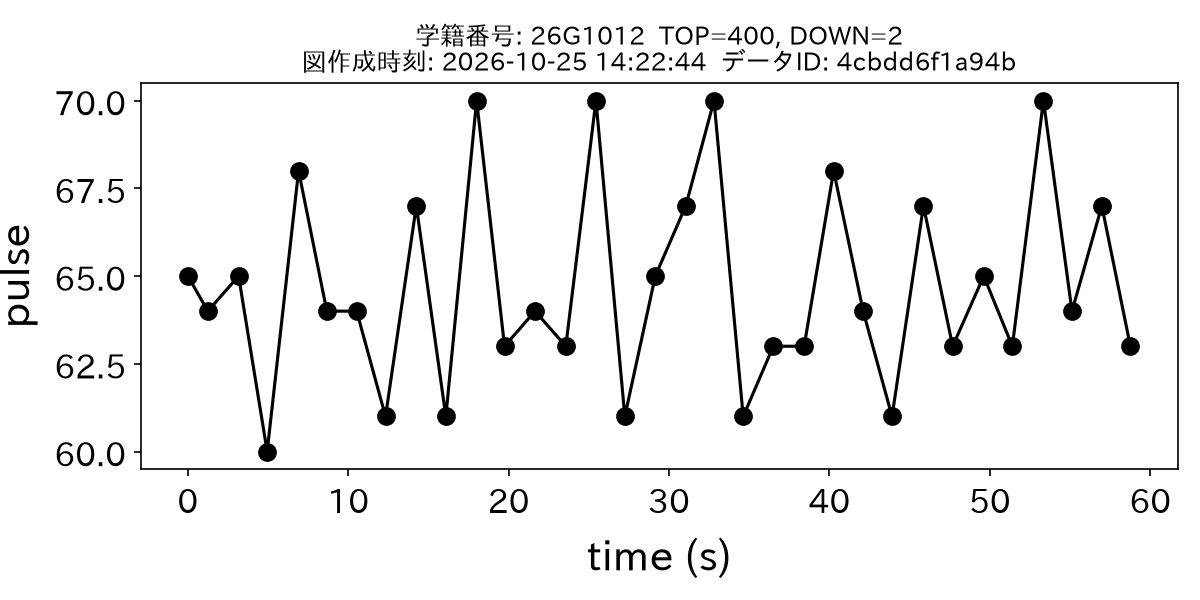
\includegraphics[width=0.75\textwidth]{fig_work_B/b3_26G1012_top400_down2_pulse_20261025_142244_4cbdd6f1a94b.png}
  \caption{脈拍数測定結果の時間変化（$\mathrm{TOP} = 400$, $\mathrm{DOWN} = 2$）}
  \label{fig:b3_pulse_plot}
\end{figure}

\begin{table}[htbp]
  \centering
  \caption{脈拍測定結果における基本統計値}
  \label{tab:pulse_statistics}

  \setlength{\tabcolsep}{16pt}
  \renewcommand{\arraystretch}{1.3}

  \begin{tabular}{lc}
    \hline
    統計項目                & 算出値         \\
    \hline
    最大値 [bpm]           & 67          \\
    最小値 [bpm]           & 60          \\
    平均値 [bpm]           & 64.6        \\
    中央値 [bpm]           & 65.0        \\
    標準偏差（不偏 / 標本） [bpm] & 2.88 / 2.58 \\
    \hline
  \end{tabular}
\end{table}

図\ref{fig:b3_pulse_plot}および表\ref{tab:pulse_statistics}を参照すると，計測された脈拍数は最小値 60\,bpm，最大値 67\,bpm の範囲に収まっており，平均値は 64.6\,bpm，中央値は 65.0\,bpm であった．
一般に健康な成人の安静時における正常脈拍数は 60 $\sim$ 100\,bpm（毎分60〜100回）とされており，今回の測定結果は平均値・中央値・最大値・最小値のすべてがこの正常安静時脈拍数の範囲内に位置している\cite{小林宏光2009脈拍数測定の正確さと測定時間との関係}．
このことから，ATOM Liteに記録された模擬脈波信号は安静時の成人における標準的な拍動リズム（周期約 0.90 $\sim$ 1.00\,s）を再現したものであることが確認できる．

また，表\ref{tab:pulse_statistics}において平均値（64.6\,bpm）と中央値（65.0\,bpm）の乖離が 0.4\,bpm と極めて小さく，不偏標準偏差が 2.88\,bpm（標本標準偏差 2.58\,bpm）と小さな値に抑えられている．
仮にピークの複数誤検出（$\times$多）が生じていれば周期が半減して 120\,bpm 超の異常高値が現れ，逆に検出漏れ（$\times$漏）やエラー処理不備が生じていれば 30\,bpm 付近の半減値や 0\,bpm が出力されて標準偏差が著しく増大するはずであるが，図\ref{fig:b3_pulse_plot}にはそのような外れ値は一切存在しない．
さらに，図\ref{fig:b3_pulse_plot}に見られる 60 $\sim$ 67\,bpm の緩やかな変動は，生体において呼吸に伴う自律神経（迷走神経・交感神経）活動の変調により拍動間隔が周期的に揺らぐ「呼吸性洞性不整脈（Respiratory Sinus Arrhythmia: RSA）」や，20\,msの離散サンプリングおよびシリアル通信処理に伴う数ミリ秒単位の周期量子化誤差を反映したものと解釈できる\cite{elgendi2019use}．
以上より，ワークB-2で決定した最適閾値とワークB-3の脈拍算出処理によって，安静時脈拍が正確に計測できていることが確認された．

\subsection{実装内容}
% ファイルごとにプログラムを記載し，変更・追加した処理について説明すること（ipynbファイルは必要ない）
% 変更しなかったファイルについては，変更していないことを説明すること

ワークB-3の実装プログラムをソースコード\ref{b3_pulse_measurement}，\ref{b3_myPulse.h}，\ref{b3_myPulse.cpp_top}，および\ref{b3_myPulse.cpp_rate}に示す．

\paragraph{b3\_pulse\_measurement.ino（ソースコード\ref{b3_pulse_measurement}）：}
配布された初期プログラムでは，\texttt{setup}関数でシリアル通信の開始のみを行い，\texttt{loop}関数で \texttt{rate()} を呼び出すだけで戻り値の出力や時間制限が未実装であったため，以下の変更・追加を行った：
\begin{itemize}
  \item \textbf{CSVヘッダー行の初期出力処理の追加}（5行目）：プログラム実行時に \texttt{time,pulse} という文字列を改行付きで1度だけシリアル出力する仕様（仕様2）を満たすため，\texttt{setup}関数内に \texttt{Serial.println("time,pulse");} を追加した．
  \item \textbf{起動後1分間の測定時間制限の実装}（9--10行目，17行目）：起動後1分が経過した場合は \texttt{rate} 関数を呼び出さないようにする仕様（仕様4）を満たすため，\texttt{loop}関数内で \texttt{float t = millis() / 1000.0;} により起動からの経過時間（秒）を算出し（9行目），\texttt{if (t < 60.0)} の条件分岐（10行目，17行目）によって60秒未満の間のみ測定処理を実行するように変更した．
  \item \textbf{エラー値の除外と経過時間・脈拍数のCSV形式出力}（11--16行目）：\texttt{rate()} 関数から返された脈拍数を変数 \texttt{v} で受け取り（11行目），ピーク検出失敗時（戻り値 \texttt{0}）にグラフへ異常値 \texttt{0} が出力されるのを防ぐため，\texttt{if (v > 0)} の条件判定（12行目）を設けた．有効な脈拍数が得られた場合のみ，\texttt{Serial.print(t, 2);}，\texttt{Serial.print(",");}，\texttt{Serial.println(v);} により経過時間（秒単位，小数点以下2桁）と脈拍数をカンマ区切りで1行ずつ出力するように実装した（13--15行目，仕様3）．
\end{itemize}

\paragraph{myPulse.h（ソースコード\ref{b3_myPulse.h}）：}
配布されたファイルから変更は行っておらず，\texttt{uint16\_t top();} および \texttt{uint8\_t rate();} の関数宣言をそのまま使用した．

\paragraph{myPulse.cpp（ソースコード\ref{b3_myPulse.cpp_top}，\ref{b3_myPulse.cpp_rate}）：}
配布時の \texttt{myPulse.cpp} では，閾値が \texttt{0} のままであり，また \texttt{rate()} 関数の中身が空（\texttt{return 0;} のみ）であったため，以下の変更および追加を行った（1ページに収めるため，前半の \texttt{top} 関数部分をソースコード\ref{b3_myPulse.cpp_top}，後半の \texttt{rate} 関数部分をソースコード\ref{b3_myPulse.cpp_rate}に分割して掲載する）：
\begin{itemize}
  \item \textbf{最適閾値の反映と \texttt{top} 関数の利用}（ソースコード\ref{b3_myPulse.cpp_top}の6--7行目，11--51行目）：ワークB-2で決定した最適閾値に従い，\texttt{TOP\_THRESHOLD} を \texttt{0} から \texttt{400} に（6行目），\texttt{DOWN\_THRESHOLD} を \texttt{0} から \texttt{2} に（7行目）変更した．なお，ワークB-3の \texttt{top()} 関数（11--51行目）はシリアル出力を行わずにピーク値のみを返す実装として完成しているため，配布コードから変更せずそのまま使用した．
  \item \textbf{2回連続のピーク検出と検出失敗時のエラー処理}（ソースコード\ref{b3_myPulse.cpp_rate}の53--63行目）：2点のピーク間隔から拍動周期を求めるため，\texttt{rate()} 関数内で \texttt{top()} 関数を2回呼び出し，1回目のピーク検出直後の時刻 \texttt{t1 = millis()}（57行目）と2回目のピーク検出直後の時刻 \texttt{t2 = millis()}（61行目）を取得した．2回連続で正しくピークが検出される必要があるため，1回目または2回目の \texttt{top()} の戻り値（\texttt{p1}, \texttt{p2}）が \texttt{0}（検出失敗）であった場合（56行目，60行目），あるいは時刻逆転等の異常時（\texttt{if (t2 <= t1)}，63行目）には，直ちに \texttt{return 0;} として測定をやり直すエラー処理を実装した．また，結合課題での誤動作を防ぐため，時刻保持に \texttt{static} 変数やグローバル変数を使用せず，関数内のローカル変数のみで完結させた．
  \item \textbf{拍動周期からの脈拍数（bpm）の算出}（ソースコード\ref{b3_myPulse.cpp_rate}の65--68行目）：2回のピーク検出時刻の差分から拍動周期 \texttt{uint32\_t period = t2 - t1;}（ミリ秒単位）を計算し（65行目），1分間（60000ミリ秒）を周期で除算した \texttt{float bpm = 60000.0 / period;} により1分間あたりの拍動回数を算出した上で（66行目），\texttt{0.5} を加算して \texttt{uint8\_t} 型へキャストすることで四捨五入した整数脈拍数を返す処理を実装した（68行目，仕様1）．
\end{itemize}

\begin{figure}[H]
  \begin{lstlisting}[caption=b3\_pulse\_measurement.ino, label=b3_pulse_measurement, escapechar=\@]
#include "myPulse.h"

void setup() {
  Serial.begin(115200);
  Serial.println("time,pulse");
}

void loop() {
  float t = millis() / 1000.0;
  if (t < 60.0) {
    uint8_t v = rate();
    if (v > 0) {
      Serial.print(t, 2);
      Serial.print(",");
      Serial.println(v);
    }
  }
}
    \end{lstlisting}
\end{figure}

\begin{figure}[H]
  \begin{lstlisting}[caption=myPulse.h, label=b3_myPulse.h, escapechar=\@]
#ifndef MyPulse_h
#define MyPulse_h

#include <Arduino.h>

uint16_t top();  // ピークを検出する
uint8_t rate();  // 脈拍を測定し返す

#endif
    \end{lstlisting}
\end{figure}

\begin{figure}[H]
  \begin{lstlisting}[caption=myPulse.cpp（前半：top関数によるピーク検出処理）, label=b3_myPulse.cpp_top, escapechar=\@]
#include "myPulse.h"

#define PIN_IN A0      // アナログ入力PINの設定
#define DELAY_TIME 20  // ディレイ時間(ms)の設定

#define TOP_THRESHOLD 400  // 信号が山の部分にあるかの判定に利用する閾値
#define DOWN_THRESHOLD 2   // 下降傾向にあるかの判定に利用する閾値
#define UP_THRESHOLD 1     // 上昇傾向にあるかの判定に利用する閾値

// アナログ入力で読み込んだ信号からピークを検出する関数
uint16_t top() {
  uint16_t maximum = 0;       // 最大値の保存用
  uint16_t value = 0;         // 読み込んだ信号の保存用
  uint8_t up_count = 0;       // 上昇傾向を判定するためのカウント
  uint8_t down_count = 0;     // 下降傾向を判定するためのカウント
  uint8_t timeout = 255;      // タイムアウトまでのカウント
  bool peak_started = false;  // 上昇傾向にあると判定されたか

  while (timeout--) {
    value = analogRead(PIN_IN);  // アナログ入力で値を読み取る

    if (value >= TOP_THRESHOLD) {  // 読み込んだ値が山の閾値以上である場合のみピーク検出の処理を行う
      if (value > maximum) {       // 読み込んだ値が最大値より大きい場合，maximum, up_count, down_countを更新する
        maximum = value;           // 最大値（maximum）を更新する
        up_count++;                // 最大値が更新されたため，up_countを増やす
        down_count = 0;            // 最大値が更新されたため，down_countを初期化する
      } else {
        down_count++;  // 最大値を更新しなかったため，down_countを増やす
      }
    }

    // up_countがUP_THRESHOLDより大きい場合，上昇傾向にあると判定する
    if (up_count > UP_THRESHOLD) peak_started = true;

    // TOP_THRESHOLD未満になり，上昇傾向と判定されていない場合は，次の山を探し直す
    if (value < TOP_THRESHOLD && !peak_started) {
      maximum = 0;
      up_count = 0;
      down_count = 0;
    }

    // 上昇傾向と下降傾向の両方を確認できた場合，ピーク値を返す
    if (peak_started && down_count > DOWN_THRESHOLD) return maximum;

    // 下降傾向を確認する前にTOP_THRESHOLD未満になった場合は，検出失敗とする
    if (value < TOP_THRESHOLD && peak_started) return 0;

    delay(DELAY_TIME);
  }
  return 0;  // timeout回数までにピークが見つからなかったら0を返す
}
    \end{lstlisting}
\end{figure}

\begin{figure}[H]
  \begin{lstlisting}[caption=myPulse.cpp（後半：rate関数による脈拍算出処理）, label=b3_myPulse.cpp_rate, firstnumber=53, escapechar=\@]
// 脈拍を測定し返す関数
uint8_t rate() {
  uint16_t p1 = top();
  if (p1 == 0) return 0;
  uint32_t t1 = millis();

  uint16_t p2 = top();
  if (p2 == 0) return 0;
  uint32_t t2 = millis();

  if (t2 <= t1) return 0;

  uint32_t period = t2 - t1;
  float bpm = 60000.0 / period;

  return (uint8_t)(bpm + 0.5);
}
    \end{lstlisting}
\end{figure}
